%%%%%%%%%%%%%%%%%%%%%%%%%%%%%%%%%%%%%%%%%
% fphw Assignment
% LaTeX Template
% Version 1.0 (27/04/2019)
%
% This template originates from:
% https://www.LaTeXTemplates.com
%
% Authors:
% Class by Felipe Portales-Oliva (f.portales.oliva@gmail.com) with template 
% content and modifications by Vel (vel@LaTeXTemplates.com)
%
% Template (this file) License:
% CC BY-NC-SA 3.0 (http://creativecommons.org/licenses/by-nc-sa/3.0/)
%
%%%%%%%%%%%%%%%%%%%%%%%%%%%%%%%%%%%%%%%%%

%----------------------------------------------------------------------------------------
%	PACKAGES AND OTHER DOCUMENT CONFIGURATIONS
%----------------------------------------------------------------------------------------

\documentclass[
	12pt, % Default font size, values between 10pt-12pt are allowed
	%letterpaper, % Uncomment for US letter paper size
	%spanish, % Uncomment for Spanish
]{fphw}

% Template-specific packages
\usepackage[utf8]{inputenc} % Required for inputting international characters
\usepackage[T1]{fontenc} % Output font encoding for international characters
\usepackage{mathpazo} % Use the Palatino font

\usepackage{graphicx} % Required for including images

\usepackage{booktabs} % Required for better horizontal rules in tables

\usepackage{listings} % Required for insertion of code

\usepackage{enumerate} % To modify the enumerate environment

\usepackage{graphicx}
\graphicspath{ {./home/vamsi/Desktop/Course Work/Labs/HPC Lab/A1_Chinnapareddy_2220570
/} }


%----------------------------------------------------------------------------------------
%	ASSIGNMENT INFORMATION
%----------------------------------------------------------------------------------------

\title{Assignment \#1} % Assignment title

\author{Chinnapareddy Krishna Vamsi \newline Roll No: 2220570} % Student name

\institute{National Institute of Technology Karnataka, Surathkal} % Institute or school name

\class{High Performance Computing(CS701)} % Course or class name

\professor{Dr. Biswajit R Bhowmik} % Professor or teacher in charge of the assignment

%----------------------------------------------------------------------------------------

\begin{document}

\maketitle % Output the assignment title, created automatically using the information in the custom commands above

%----------------------------------------------------------------------------------------
%	ASSIGNMENT CONTENT
%----------------------------------------------------------------------------------------

\section*{Latex}

\textbf{Objective: } To explore various latex functionalities for making a report.

\begin{problem}
	Latex Introduction
\end{problem}
\begin{center}
	
\includegraphics[width=0.5\columnwidth]{LaTeX_logo.png} % Example image
\end{center}

%------------------------------------------------

\subsection*{}

In this report, we will go through the basics of using LATEX. LATEX is a tool used to create professional-looking documents. It creates beautifully typeset documents and allows users to efficiently tackle the more complicated parts of typesetting, such as inputting mathematics, creating tables of contents, referencing, and adding images, and having a consistent layout across all sections.

%----------------------------------------------------------------------------------------

\subsection*{}
Let's see how to write basic \lstinline!\LaTeX! code 

\begin{lstlisting}
\documentclass{article}
\begin{document}
This is my first latex document
\end{document}
\end{lstlisting}

Output:

\begin{center}

\includegraphics[width=7cm, height=4cm]{Image1}
\end{center}


\subsection*{}
You can see that LATEX has already taken care of the first piece of formatting for you, by indenting the first line of the paragraph. Let's have a close look at what each part of our code does.

The first line of code declares the type of document, known as the class. The class controls the overall appearance of the document. Different types of documents will require different classes i.e. a CV/resume will require a different class than a scientific paper. In this case, the class is article, the simplest and most common LATEX class. Other types of documents you may be working on may require different classes such as book or report.

After this, you write the content of our document, enclosed inside the begin document and end document tags. This is known as the body of the document. You can start writing here and make changes to the text if you wish. To see the result of these changes in the PDF you have to compile the document.

%%%%%%%%%%%%%%%%%%%%%%%%%%%%%%%%%%%%%%%%%%%% Preamble %%%%%%%%%%%%%%%%%%%%%%%%%%%%%%%%%%%%

\begin{problem}
	Preamble of a document
\end{problem}

\subsection*{}
In the previous example the text was entered after the begin document command. Everything in your .tex file before this point is called the preamble. In the preamble you define the type of document you are writing, the language you are writing in, the packages you would like to use (more on this later) and several other elements. For instance, a normal document preamble would look like this:

\begin{lstlisting}
\documentclass{article}
\end{lstlisting}

%%%%%%%%%%%%%%%%%%%%%%%%%%%%%%%%%%%%%% Adding a title, author and date %%%%%%%%%%%%%%%%%%%%%%%%%%%%%%

\begin{problem}
	Adding a title, author and date
\end{problem}

\subsection*{}
To add a title, author and date to our document, you must add below mentioned lines to the preamble. With these lines added, your preamble should look something like this

\begin{lstlisting}
\title{Assignment \#1} % Assignment title

\author{Chinnapareddy Krishna Vamsi} % Student name

\institute{National Institute of Technology Karnataka, Surathkal} % Institute name

\class{High Performance Computing(CS701)} % Course or class name

\professor{Dr. Biswajit R Bhowmik} % Professor or teacher in charge of the assignment

\date{Sep 2022}
\end{lstlisting}

Output:

\begin{center}

\includegraphics[width=10cm, height=7cm]{Image2}
\end{center}


%%%%%%%%%%%%%%%%%%%%%%%%%%%%%%%%% Adding Image %%%%%%%%%%%%%%%%%%%%%%%%%%%%%%%%%%%%

\begin{problem}
	Adding Image to a latex document.
\end{problem}

\subsection*{}
Let's see how to add image to a latex document.

\begin{lstlisting}
\documentclass{article}
\usepackage{graphicx}
\graphicspath{ {./images/} }
 
\begin{document}

\includegraphics{HPC}

\end{document}
\end{lstlisting}

Output:

\begin{center}
\includegraphics[scale = 0.3]{HPC}
\end{center}


We use the graphicx package to manage images in LaTeX. The place where the images are kept is denoted by the command  graphicspath curlybraces ./images/ curlybraces. The folder “images” is under the directory of the main document.

The  includegraphics sun  command includes the image named "HPC" in the document. Here, we have not added any extension or the image format to the name. Also, the name of the file should not contain white spaces or multiple dots.

Please note that the file extension can be included, but it is usually recommended to omit it. This way, LaTeX will search all the supported format for that file within the folder.

%%%%%%%%%%%%%%%%%%%%%%%%%%%%%%%%% Adding Table %%%%%%%%%%%%%%%%%%%%%%%%%%%%%%%%%%%%

\begin{problem}
	Create Table in latex document.
\end{problem}

\subsection*{}
The tables are common feature used in academic writing. This section will explain the steps to create the table. Tables are an efficient way to represent the information and are often used in most of the documents or files. When discussing the scientific papers, the tables are used to present the data. Creating the table in Latex is a little complicated compared to others. But here, the steps and the process to create a table from the basics will make the process easier.
\newline\newline
The commands used to create table are:

\begin{lstlisting}
\documentclass{article}  
\begin{document}  
\begin{center}  
\begin{tabular}{|l|c|r|}  
\hline  
a&b&c\\ \hline  
d&e&f\\ \hline  
g&h&i\\ \hline  
\end{tabular}  
\end{center}  
\end{document}
\end{lstlisting}

Output:
\begin{center}
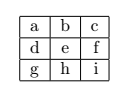
\includegraphics[scale = 0.5]{Table}
\end{center}


Here, the table signifies the tabular environment, together with the caption command. The command where is used to determine the location for the table. For example, begin table  t  means, the table will appear at the top of the page.
\newline\newline
The tabular environment uses ampersands symbol for the column separation.
\newline\newline
The letters used to align the content to the left, center, and right are l, c, and r for each of the columns. The command passed for aligning is begin tabular  l c r .
\newline\newline
The command used to draw vertical lines separating the columns of the table is begin tabular l|c|r, where the (|) is passed as an argument. The | symbol is used to draw the vertical lines between the columns.
\newline\newline
You can also use the vline command to draw vertical lines. The vline command draws the vertical line along with the height of the row.

%%%%%%%%%%%%%%%%%%%%%%%%%%%%%%%%% Adding Math %%%%%%%%%%%%%%%%%%%%%%%%%%%%%%%%%%%%

\begin{problem}
	Adding mathematical symbols in latex document.
\end{problem}

\subsection*{}
The default version of LaTeX may lack some of the functionalities or features. For example, Trimming or Overlapping of equations when equations are very long. To overcome these challenges, you can use the "asmmath" package.
\newline\newline
Check the below example to understand:

\begin{lstlisting}
\begin{equation} \label{equation1}
\begin{split}
Area & = \frac{length \times breadth }{2} \\
     & = \frac{1}{2} length \times breadth
\end{split}
\end{equation}

\end{lstlisting}

Output:

\begin{center}
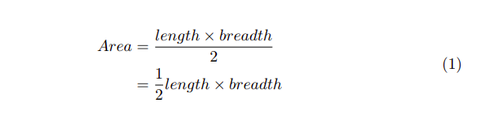
\includegraphics[scale = 0.5]{Math}
\end{center}

As shown in the example above, utilize the split environment if you would like to split the equations into smaller parts. The split environment will align these smaller parts. Make usage of ampersand character in order to align the equations vertically. Double backslash provides the functionality of newline character.

%%%%%%%%%%%%%%%%%%%%%%%%%%%%%%%%% Fonts %%%%%%%%%%%%%%%%%%%%%%%%%%%%%%%%%%%%

\begin{problem}
	Latex Fonts Size and Styles.
\end{problem}

\subsection*{}
We usually define the paper size and the font size inside the square brackets []. The point size can be described in the way [10pt]. The other font sizes are 8pt, 9pt, 10pt, 11pt, 12pt, 14pt, 17pt, 20pt. The default font size for Latex is 10pt.
\newline\newline
LaTeX normally chooses the appropriate font and font size based on the logical structure of the document (e.g. sections). In some cases, you may want to set fonts and sizes by hand.
\newline\newline
The following example shows how to use the smallest available font size in LaTeX backslash tiny and the small caps backslash textsc font style:
\newline\newline

\begin{lstlisting}
This is a simple example, {\tiny this will show different font sizes} and also \textsc{different font styles}.
\end{lstlisting}

Output:

\begin{center}

\includegraphics[scale = 0.5]{fonts1}
\end{center}

Typefaces usually come in various styles and weights, such as italic and bold. The following table lists the commands you will need to access typical font shapes.
\newline\newline

\begin{center}
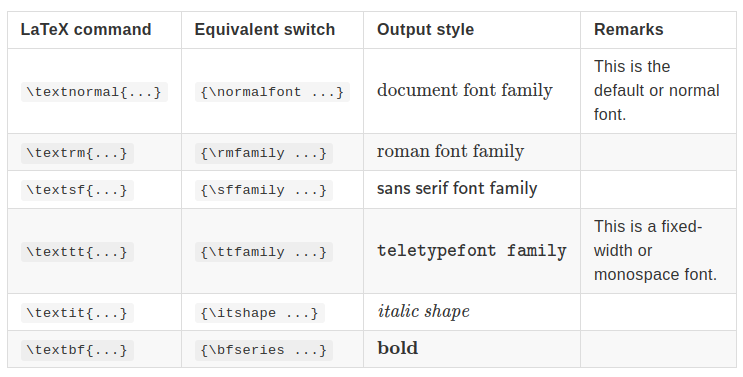
\includegraphics[scale = 0.5]{fonts2}
\end{center}

\end{document}